\documentclass[a4paper,english,cleveref, autoref]{lipics-v2019}
% ECOOP 2020: 25 pages excluding references
%This is a template for producing LIPIcs articles. 
%See lipics-manual.pdf for further information.
%for A4 paper format use option "a4paper", for US-letter use option "letterpaper"
%for british hyphenation rules use option "UKenglish", for american hyphenation rules use option "USenglish"
%for section-numbered lemmas etc., use "numberwithinsect"
%for enabling cleveref support, use "cleveref"
%for enabling cleveref support, use "autoref"

\usepackage{pgfplots}
\usepackage{tikz}
\usetikzlibrary{positioning}

\newcommand{\NPM}{NPM}
\newcommand{\NodeJS}{NodeJS}

% Result numbers: Check `numbers.log` in `dts-generate-results' repo
\newcommand{\CountTotalModulesDefinitelyTyped}{6029}
\newcommand{\CountModulesWithRepositoryUrl}{4974}
\newcommand{\CountModulesWithReadmeFile}{4292}
\newcommand{\CountModulesWithCodeExamples}{2260}
\newcommand{\CountModulesWorkingCodeExamples}{946}
\newcommand{\CountModulesRunTimeInfoExtracted}{436}
\newcommand{\CountModulesGeneratedDeclarationFile}{249}
\newcommand{\CountModulesOnlySolvableDifferences}{111}

% Result helper numbers
\newcommand{\CountModulesWithoutReadmeFile}{682} % \CountModulesWithRepositoryUrl{} - \CountModulesWithReadmeFile{}
\newcommand{\CountModulesNotWorkingCodeExamples}{1314} % \CountModulesWithCodeExamples{} - \CountModulesWorkingCodeExamples{}
\newcommand{\CountModulesRunTimeInfoCouldNotBeExtracted}{510} % \CountModulesWorkingCodeExamples{} - \CountModulesRunTimeInfoExtracted{}
\newcommand{\CountModulesDeclarationFileCouldNotBeGenerated}{138} % \CountModulesGeneratedDeclarationFile{} - \CountModulesOnlySolvableDifferences{}

\definecolor{backgroundgray}{rgb}{.94,.94,.94}
\definecolor{lightgray}{rgb}{.35,.35,.5}
\definecolor{darkgray}{rgb}{.2, .2, .2}
\definecolor{purple}{rgb}{0.65, 0.12, 0.82}

\newcommand{\secref}[1]{Section~\ref{#1} - \nameref{#1}}
\newcommand{\figref}[1]{Figure~\ref{#1}}
\newcommand{\coderef}[1]{Listing~\ref{#1}}

\lstdefinelanguage{JavaScript}{
  keywords={typeof, new, true, false, catch, function, return, null, catch, switch, var, if, in, while, do, else, case, break, undefined},
  keywordstyle=\color{black}\bfseries,
  ndkeywords={class, export, boolean, throw, implements, import, this},
  ndkeywordstyle=\color{black}\bfseries,
  identifierstyle=\color{darkgray},
  sensitive=false,
  comment=[l]{//},
  morecomment=[s]{/*}{*/},
  commentstyle=\color{lightgray}\slshape,
  stringstyle=\color{darkgray}\ttfamily,
  morestring=[b]',
  morestring=[b]"
}

\lstdefinelanguage{TypeScript}{
  keywords={typeof, new, true, false, catch, function, return, null, catch, switch, var, if, in, while, do, else, case, break, undefined},
  keywordstyle=\color{black}\bfseries,
  ndkeywords={class, export, boolean, throw, implements, import, this, declare, constructor, namespace, interface},
  ndkeywordstyle=\color{black}\bfseries,
  identifierstyle=\color{darkgray},
  sensitive=false,
  comment=[l]{//},
  morecomment=[s]{/*}{*/},
  commentstyle=\color{lightgray}\slshape,
  stringstyle=\color{darkgray}\ttfamily,
  morestring=[b]',
  morestring=[b]"
}

\lstset{
   backgroundcolor=\color{backgroundgray},
   extendedchars=true,
   basicstyle=\footnotesize\ttfamily,
   showstringspaces=false,
   showspaces=false,
   numbers=left,
   numberstyle=\footnotesize,
   numbersep=9pt,
   tabsize=2,
   breaklines=true,
   showtabs=false
}

\graphicspath{{./graphics/}}%helpful if your graphic files are in another directory

\bibliographystyle{plainurl}% the mandatory bibstyle

\title{Generation of TypeScript Declaration Files from JavaScript Code}

% \titlerunning{Dummy short title}%optional, please use if title is longer than one line

\author{John Q. Public}{Dummy University Computing Laboratory, Country \and My second affiliation, Country \and \url{http://www.myhomepage.edu} }{johnqpublic@dummyuni.org}{https://orcid.org/0000-0002-1825-0097}{(Optional) author-specific funding acknowledgements}%TODO mandatory, please use full name; only 1 author per \author macro; first two parameters are mandatory, other parameters can be empty. Please provide at least the name of the affiliation and the country. The full address is optional

\authorrunning{J.\,Q. Public}%TODO mandatory. First: Use abbreviated first/middle names. Second (only in severe cases): Use first author plus 'et al.'

\Copyright{John Q. Public}%TODO mandatory, please use full first names. LIPIcs license is "CC-BY";  http://creativecommons.org/licenses/by/3.0/

\ccsdesc[300]{Software and its engineering~Software notations and tools}
\ccsdesc[100]{Software and its engineering~General programming languages}%TODO mandatory: Please choose ACM 2012 classifications from https://dl.acm.org/ccs/ccs_flat.cfm 

\keywords{JavaScript, TypeScript, Dynamic Analysis, Declaration Files}%TODO mandatory; please add comma-separated list of keywords

\category{}%optional, e.g. invited paper

\relatedversion{}%optional, e.g. full version hosted on arXiv, HAL, or other repository/website
%\relatedversion{A full version of the paper is available at \url{...}.}

\supplement{}%optional, e.g. related research data, source code, ... hosted on a repository like zenodo, figshare, GitHub, ...

%\funding{(Optional) general funding statement \dots}%optional, to capture a funding statement, which applies to all authors. Please enter author specific funding statements as fifth argument of the \author macro.

% \acknowledgements{I want to thank \dots}%optional

%\nolinenumbers %uncomment to disable line numbering

%\hideLIPIcs  %uncomment to remove references to LIPIcs series (logo, DOI, ...), e.g. when preparing a pre-final version to be uploaded to arXiv or another public repository

%Editor-only macros:: begin (do not touch as author)%%%%%%%%%%%%%%%%%%%%%%%%%%%%%%%%%%
\EventEditors{John Q. Open and Joan R. Access}
\EventNoEds{2}
\EventLongTitle{42nd Conference on Very Important Topics (CVIT 2016)}
\EventShortTitle{CVIT 2016}
\EventAcronym{CVIT}
\EventYear{2016}
\EventDate{December 24--27, 2016}
\EventLocation{Little Whinging, United Kingdom}
\EventLogo{}
\SeriesVolume{42}
\ArticleNo{23}
%%%%%%%%%%%%%%%%%%%%%%%%%%%%%%%%%%%%%%%%%%%%%%%%%%%%%%

\begin{document}

\maketitle

%TODO mandatory: add short abstract of the document
\begin{abstract}
Developers are starting to write large and complex applications in
TypeScript, a typed dialect of JavaScript. TypeScript applications
integrate JavaScript libraries via typed descriptions of their APIs
called declaration files. DefinitelyTyped is the standard public
repository for these files.
The repository is maintained manually by volunteers, which
is error prone and time consuming. Discrepancies between a
declaration file and the JavaScript implementation lead to
incorrect feedback from the TypeScript IDE and thus to incorrect uses
of the underlying JavaScript library.

This work presents \texttt{dts-generate}, a tool that generates
TypeScript declaration files for JavaScript libraries uploaded to the \NPM{}
registry. It extracts code examples from the documentation written by
the developer, executes the library driven by the examples, gathers
run-time information, and generates a declaration file based on this
information. To evaluate the tool, 244 declaration files were generated and 82 were
compared with the corresponding declaration file provided on DefinitelyTyped. 72 files presented positive results, having no differences at all or differences that can be solved by modifying the code examples accordingly.

\end{abstract}

\section{Introduction}
\label{sec:introduction}
JavaScript has become the most popular language for writing web
applications \cite{github-statistics}. It is also gaining popularity
for back-end applications running in \NodeJS{}, a JavaScript-based
server-side platform. JavaScript is appealing to developers because
its forgiving dynamic typing enables 
them to create simple pieces of code very quickly and proceed on a
trial-and-error basis.

JavaScript was never intended to be more than a
scripting language. Hence, it lacks features for maintaining and evolving large
codebases.
Presently, however, JavaScript is being used for creating large and complex
applications. 
Mistakes such as mistyped property
names and misunderstood or unexpected type coercions cause developers
to spend a significant amount of time in debugging. There is ample
evidence for such mishaps. For example, a 
JavaScript code blog\footnote{\url{https://wtfjs.com}} collects experiences
from developers facing unexpected situations while programming in
JavaScript. \coderef{code:introduction-javascript-wtfs} exposes some
of these unintuitive JavaScript behaviors. 

\begin{lstlisting}[
    caption={\textbf{Unintuitive JavaScript behavior} - falsy values, \lstinline!typeof!, \lstinline!null! and \lstinline!undefined! operators and type coercion},
    language=JavaScript,
	label=code:introduction-javascript-wtfs,
    float,
    abovecaptionskip=-\medskipamount
]
"0" == false; // true
true == "1.00"; // true
false == "    \n\r\t     "; // true
false == []; // true
0 == []; // true
null == undefined; // true
[1] + 1; //'11'
[2] == "2"; // true
null + undefined + [1, 2, 3] // 'NaN1,2,3'
"hello world".lenth + 1 // NaN | note 'lenth' instead of 'length'
[1, 15, 20, 100].sort() // [ 1, 100, 15, 20 ]
typeof null; // object
null instanceof Object; // false
"01" < "00100"; // false
\end{lstlisting}
% pjt: why unexpected?

The cognitive load produced by such dynamic typing (which includes
unchecked property names) is not present in other languages that use
build tools based on type information. This insight motivated the
creation of TypeScript, a superset of JavaScript with type
annotations \cite{typescript}. It has become a widely used alternative
among JavaScript developers, because it incorporates features that are
helpful for developing and maintaining large applications
\cite{DBLP:conf/icse/GaoBB17}. TypeScript enables the early detection
of several kinds of run-time errors and the integration of code intelligence
tools like auto-completion in an IDE.

Existing JavaScript libraries can be used in a TypeScript project by
adding a declaration file that contains a description of the library's
API in terms of types. Lots of declaration files for popular
JavaScript libraries have been created in a community effort in the
DefinitelyTyped repository~\cite{definitely-typed-repository}.
At the time of writing this repository contains declaration files for
more than 6000 JavaScript libraries. Unfortunately, most declaration
files in this libraries have been manually created and maintained,
which is error prone and time consuming. As TypeScript takes a
declaration file at face value, discrepancies are not detected at
compile time and the inaccurate code-intelligence features are misleading the
programmer. Moreover, TypeScript does not perform any run-time 
checking on types, either, so that a discrepancy  between the declaration file
and its corresponding JavaScript library can lead to unexpected 
behavior and crashes. Such behavior can lead to developer
frustration, longish debugging sessions, and decreasing confidence in
the tool chain.

Some previous work tackled the problem of improving the quality of
declaration files. Feldthaus et al
\cite{DBLP:conf/oopsla/FeldthausM14} search automatically for
mismatches between a declaration file and implementation code. TSTest
\cite{DBLP:journals/pacmpl/KristensenM17}
adapted feedback-directed random testing to detect discrepancies between a
declaration file and a JavaScript library. Tools like TSInfer and
TSEvolve~\cite{DBLP:conf/fase/KristensenM17} are designed for
assisting the creation of new declaration 
files and supporting the evolution the declaration file when the
corresponding JavaScript library gets modified, respectively. They
rely on an existing static analyzer for JavaScript \cite{TAJS}.
TypeScript itself
developed \texttt{dts-gen}, a tool that generates a
declaration file that is meant to be used as a \emph{starting point
for writing a high-quality declaration file} \cite{dts-gen}.

In this work we present the tool \texttt{dts-generate}
as a first step to explore the possibilities for
generating useful declaration files without the heavy lifting of
static analysis. \texttt{dts-generate} comes with a framework that
supports the generation of declaration files for an existing
JavaScript library published to the \NPM{} registry. The tool gathers
data flow and type information at run-time to generate a declaration
file based on that information.

The novelty of our tool is twofold:
\begin{enumerate}
\item 
  We do not rely on static analysis, which is hard to implement
  soundly and precisely and which is prone to maintenance problems
  when keeping up with JavaScript's yearly language updates.
\item
  Instead we extract example code from the programmer's library
  documentation and rely on dynamic analysis to extract typed usage
  patterns for the library from the example runs.
\end{enumerate}
% The architecture supports the future incorporation of a Symbolic
% Execution Engine that expands the initial code base using the
% signatures in the declaration file. The iterative process of exploring
% new execution paths will refine the generated declaration file in each
% iteration. 

% Finally, we generated declaration files for 244 JavaScript libraries
% and evaluated them against the DefinitelyTyped repository. 

The contributions of this paper are as follows.
\begin{itemize}
% \item We introduce an architecture that supports generating TypeScript
%   Declaration Files for a given JavaScript Library using run-time
%   information. The architecture supports the future incorporation of a
%   Symbolic Execution Engine that expands the initial code base using
%   the signatures in the declaration file. The iterative process of
%   exploring new execution paths will refine the generated declaration
%   file in each iteration.
\item A framework that extracts code examples from the
  documentation of an \NPM{} package and collects run-time type
  information from running these examples.

\item The tool \texttt{dts-generate}, a command line
  application that generates a valid TypeScript declaration file for a
  specific \NPM{} package using run-time information.

\item A comparator for TypeScript declaration files. This tool is
  necessary for evaluating our framework and also useful to detect
  incompatibilities when evolving JavaScript modules.
\item An evaluation of our framework. We examined all 6029 entries in
  the DefinitelyTyped repository and found 244 sufficiently
  well-documented \NPM{} packages, on which we ran \texttt{dts-generate}
  and compared the outcome with the respective declaration file from the
  DefinitelyTyped repository. 

\end{itemize}

\section{Motivating Example}
\label{sec:motivating-example}
The \NPM{} package \texttt{glob-to-regexp} is a simple JavaScript library, which turns a glob expression into a regular expression\footnote{https://www.npmjs.com/package/glob-to-regexp}. It
has about 6,500,000 weekly downloads and 181 \NPM{} packages depend on it. If
a developer creates or extends TypeScript code that depends on the
\texttt{glob-to-regexp} library, the TypeScript
compiler and IDE requires a declaration file for that library to
perform static checking and code completion, respectively. We 
use \texttt{dts-generate} to automatically generate a TypeScript
declaration file for \texttt{glob-to-regexp}. The tool downloads the \NPM{} 
package, runs the examples extracted from its documentation, gathers
run-time information, and generates a TypeScript declaration
file. The result is 
shown in \figref{fig:motivating-example-glob-to-regexp-vscode} and it is
ready for use in a TypeScript project. For example,  Visual Studio's
code completion runs properly with it
(\figref{fig:motivating-example-glob-to-regexp-vscode}). If the
\texttt{glob-to-regexp} package gets modified in the future, a new declaration
file can be generated automatically using
\texttt{dts-generate}. Our comparator tool can compare the new file
for incompatibilities with the previous declaration file.

\begin{figure}[tp]
  \centering
  \begin{subfigure}{0.70\linewidth}
    \begin{lstlisting}[language=TypeScript]
export = GlobToRegexp;

declare function GlobToRegexp(glob: string, opts: undefined): RegExp;
declare function GlobToRegexp(glob: string, opts: GlobToRegexp.I__opts): RegExp;
declare namespace GlobToRegexp {
  export interface I__opts {
    'extended': undefined | boolean;
    'globstar': undefined | boolean;
    'flags': undefined | string;
  }

}
    \end{lstlisting}
  \end{subfigure}

  \hspace{10.\textwidth}

  \begin{subfigure}{1.\linewidth}
    \centering
    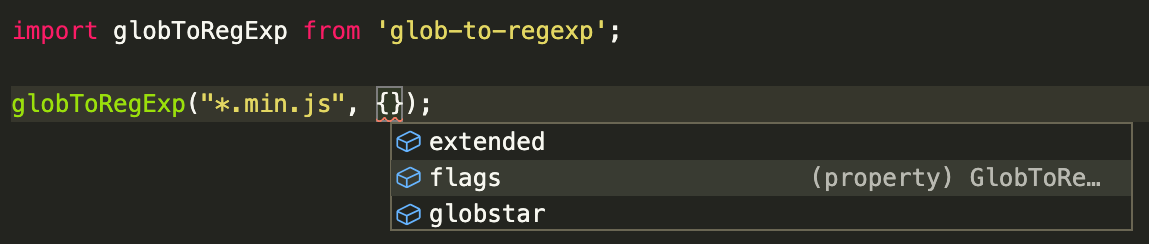
\includegraphics[width=0.8\linewidth]{motivating-example-glob-to-regexp-vscode.png}
  \end{subfigure}

  \caption{\textbf{Declaration file for \texttt{glob-to-regexp} generated with \texttt{dts-generate}} - Interfaces is correctly detected. Optional parameters are explicitly declared as \texttt{undefined}. Declaration file can be correctly used in Visual Studio Code\footnote{https://code.visualstudio.com}.}
  \label{fig:motivating-example-glob-to-regexp-vscode}
\end{figure}

After filling in some background information on declaration files,
Section~\ref{sec:gener-typescr-decl} examines each step in the
generation process in detail and refer back to this example for
concreteness.

\section{TypeScript Declaration Files}
\label{sec:typescr-decl-files}

The declaration file shown in
\figref{fig:motivating-example-glob-to-regexp-vscode} describes a
package with a single exported function. The first parameter is of type \texttt{string} and the second one is an optional interface. TypeScript namespaces are used for organizing types declared in a declaration file and avoiding name collisions with other types \cite{typescript-namespaces}. For example, the interface \texttt{I\_\_opts} declared in \figref{fig:motivating-example-glob-to-regexp-vscode} is used as \lstinline[language=TypeScript]{globToRegexp.I__opts}, since it is declared within a namespace.


This file is an instance of one of the standard templates for writing
declaration
files\footnote{https://www.typescriptlang.org/docs/handbook/declaration-files/templates.html}:
\textbf{module}, \textbf{module-class} and
\textbf{module-function}. 
Each template corresponds to a different way of describing the exports
of a JavaScript library. Choosing the template depends on the
particular organization of the underlying JavaScript library:
\begin{description}
\item[module] several exported functions,
\item[module-class] a class-like structure,
\item[module-function] exactly one exported functions.
\end{description}

\begin{lstlisting}[
    caption={Example for template \textbf{module-function}},
    language=bash,
	label=code:dts-generate-example,
    float,
    abovecaptionskip=-\medskipamount
]
$ ./dts-generate abs
$ cat output/abs/index.d.ts 
export = Abs;

declare function Abs(input: string): string;
\end{lstlisting}

TypeScript provides a guide on how to write high quality declaration files\footnote{https://www.typescriptlang.org/docs/handbook/declaration-files/by-example.html}. They explain the main concepts through examples. We extracted one example for each template and generated used \texttt{dts-generate} to generate a corresponding declaration file, as presented in \figref{fig:typescript-templates-by-example}. The \texttt{glob-to-regexp} library is an instance of a \textbf{module-function}. It is worth mentioning that templates are a way of describing how a JavaScript library is intended to be used. Although highly unlikely, it is possible to create a library that can be represented with a different template depending on how it is used, as shown in \figref{fig:multi-purpose-module-example}. Run-time analysis proves useful in this case, since it is not sufficient to statically analyze the exported module.

\begin{figure}[tp]
  \centering
  \begin{subfigure}{0.48\linewidth}
    \begin{lstlisting}[language=JavaScript]
var greet = require("./greet-settings-module");

greet({
  greeting: "hello world",
  duration: 4000
});

greet({
  greeting: "hello world",
  color: "#00ff00"
});
    \end{lstlisting}
    \caption{TypeScript example for \texttt{module-function} template}
  \end{subfigure}
  \hfill
  \begin{subfigure}{0.48\linewidth}
    \begin{lstlisting}[language=TypeScript]
export = GreetSettingsModule;

declare function GreetSettingsModule(settings: GreetSettingsModule.I__settings): void;
declare namespace GreetSettingsModule {
  export interface I__settings {
    'greeting': string;
    'duration': number | undefined;
    'color': undefined | string;
  }

}
    \end{lstlisting}
    \caption{Declaration file for \texttt{module-function} template}
  \end{subfigure}

  \begin{subfigure}{0.48\linewidth}
      \begin{lstlisting}[language=JavaScript]
var myLib = require("./greet-module");

var result = myLib.makeGreeting("hello, world");
console.log("The computed greeting is: " + result);

var goodbye = myLib.makeGoodBye();
console.log("The computed goodbye is: " + goodbye);    
      \end{lstlisting}
      \caption{Example for \texttt{module}}
    \end{subfigure}
    \hfill
    \begin{subfigure}{0.48\linewidth}
      \begin{lstlisting}[language=TypeScript]
export function makeGreeting(str: string): string;
export function makeGoodBye(): string;        
      \end{lstlisting}
      \caption{Declaration file for \texttt{module} template}
    \end{subfigure}

    \begin{subfigure}{0.48\linewidth}
      \begin{lstlisting}[language=JavaScript]
var Greeter = require("./greet-classes-module.js");

var myGreeter = new Greeter("hello, world");
myGreeter.greeting = "howdy";
myGreeter.showGreeting();
      \end{lstlisting}
      \caption{Example for \texttt{module-class}}
    \end{subfigure}
    \hfill
    \begin{subfigure}{0.48\linewidth}
      \begin{lstlisting}[language=TypeScript]
export = Greeter;

declare class Greeter {
  constructor(message: string);
  showGreeting(): void;
}

declare namespace Greeter {
}
      \end{lstlisting}
      \caption{Declaration file for \texttt{module-class} template}
    \end{subfigure}

  \caption{Results for \textbf{module-function} template}
  \label{fig:typescript-templates-by-example}
\end{figure}

\begin{figure}[tp]
  \centering
  \begin{subfigure}{0.80\linewidth}
      \begin{lstlisting}[language=JavaScript]
var multiPurposeModule = require('./multi-purpose-module');

// module-function
console.log(multiPurposeModule("John", "Doe"));
// John Doe


// module-class
var m = new multiPurposeModule("Jane", "Doe");
console.log(m.firstName + " - " + m.lastName);
// Jane - Doe

console.log(m.sayHello());
// Hello, my name is Jane Doe

// module
console.log(multiPurposeModule.anotherFunction());
// I am another function! 
      \end{lstlisting}
      \caption{index.js}
    \end{subfigure}

    \begin{subfigure}{0.80\linewidth}
      \begin{lstlisting}[language=TypeScript]
var multiPurposeModule = function(firstName, lastName) {
  this.firstName = firstName;
  this.lastName = lastName;

  return firstName + " " + lastName;
};

multiPurposeModule.prototype.sayHello = function() {
  return "Hello, my name is " + this.firstName + " " + this.lastName;
};

multiPurposeModule.anotherFunction = function() {
  return "I am another function!";
};

module.exports = multiPurposeModule;   
      \end{lstlisting}
      \caption{multi-purpose-module/index.js}
    \end{subfigure}
  \caption{Example module that implements all three templates simultaneously}
  \label{fig:multi-purpose-module-example}
\end{figure}


\section{The Generation of TypeScript Declaration Files}
\label{sec:gener-typescr-decl}
This section gives an overview of our approach to generating
TypeScript declaration files from JavaScript libraries packaged in
\NPM. \figref{fig:tsd_generation_method_block_diagram} gives a rough
picture of the inner working of our tool \texttt{dts-generate}. The
input is an \NPM{} package and the output is a TypeScript declaration
file for the package if it is ``sufficiently documented'', which we
substantiate in the next subsection.

% We introduce \texttt{dts-generate}, a command line tool which
% generates a valid TypeScript Declaration File for a specific
% JavaScript Library uploaded to the \NPM{} Registry, as explained in
% \figref{fig:tsd_generation_method_block_diagram}. The tool is intended
% to be used on existing, published \NPM{} packages. The generated
% output TypeScript declaration file is a valid file which can be used
% for development and uploaded to the DefinitelyTyped Repository. 

\begin{figure}[tp]
    \centering
    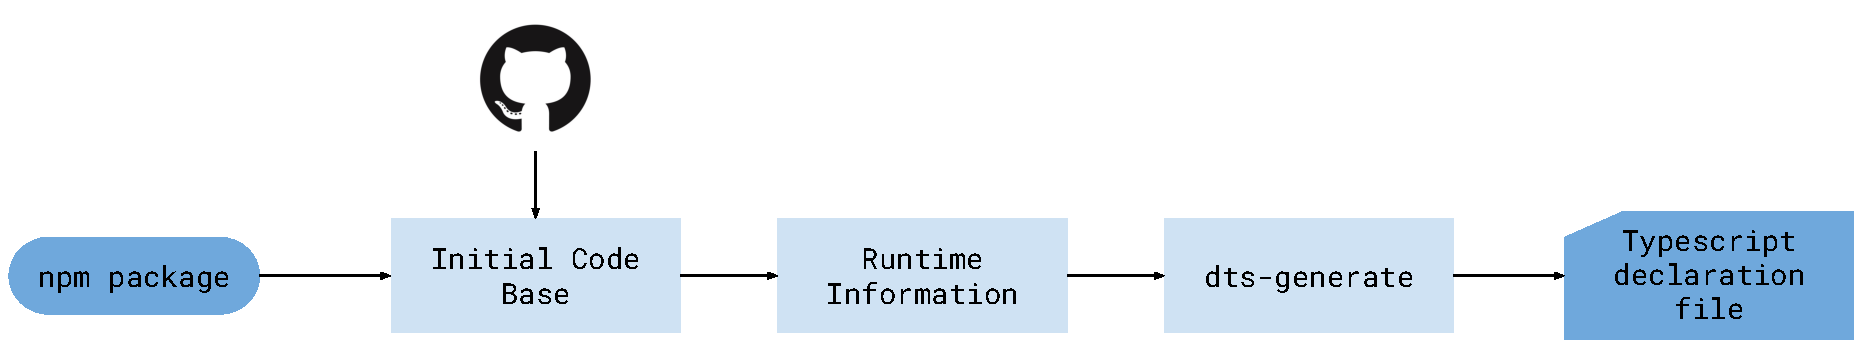
\includegraphics[width=1\linewidth]{dts-generate-block-diagram.pdf}
    \caption[dts-generate - Architecture overview]{\textbf{dts-generate - Architecture overview} - Initial code base is retrieved from the \NPM{} package's repository. A valid TypeScript Declaration File is generated using run-time information. A Symbolic Execution Engine creates test cases based on the generated Declaration File and via a feedback loop enriches the code base until the stopping criteria is reached. The final TypeScript Declaration File gets returned. Feedback loop through the Symbolic Execution Engine was not implemented. It can be added in a future to the existing architecture, without modifying the working blocks.}
    \label{fig:tsd_generation_method_block_diagram}
  \end{figure}

As \texttt{dts-generate} is based on run-time information, 
exemplary code fragments that execute the JavaScript library are
needed to obtain 
significant run-time information from running the instrumented library
code.


The examples and the code base of the library are instrumented with
Jalangi \cite{DBLP:conf/sigsoft/SenKBG13} to gather data flow
information and type information at runtime. Jalangi is a configurable
framework for dynamic analysis of JavaScript. It provides several
analysis modules that we extended as needed to retrieve the required
run-time information, which is then saved in a JSON file. 

A second independent block uses the run-time information to generate a
TypeScript declaration file. It infers the overall structure of the JavaScript
library, its interfaces, and the types from the run-time information. 
The resulting declaration file is ready for use in the development
process. Its content mimics the usage of the library in the example
code fragments and matches the structure of the
JavaScript library under analysis, so that the JavaScript code
generated after compiling the TypeScript code runs without
interface-related errors.

The command line interface is inspired by the \texttt{dts-gen} package
\cite{dts-gen}. \coderef{code:dts-generate-example} shows
that invoking the package is very simple and the only required
argument is the name of the module published to the \NPM{} registry. 


\subsection{Initial Code Base}
\label{sec:initial-code-base}

To extract run-time information from a JavaScript library, it is
necessary, by definition, to actually execute the code, because the
analysis modules provided by Jalangi to gather information are only
triggered if the instrumented code gets executed.

There are several options to obtain code fragments that drive the
library code:
\begin{enumerate}
\item\label{item:1} execute code that imports the library;
\item\label{item:2} execute the test cases that come with the library;
\item\label{item:3} execute code fragments extracted from the library documentation.
\end{enumerate}

Option~\ref{item:1} does not solve our problem, it just delegates it
to the importing library, which also needs code to drive it. Moreover,
it is costly to download and instrument another package.

We considered option~\ref{item:2} under the assumption that most
libraries would come with test cases. However, there is no standard
for testing JavaScript code so that test cases were difficult to reap
from the \NPM{} packages: they use different directory structures,
employ differing (or no) testing tools, or do not have tests
at all. Moreover, developers try to cover edge cases or even not allowed values in their tests. Such tests are not really useful for describing a library from the consumer's point of view. For example, a developer might write a test invoking a function with \texttt{null} just to validate that it throws an error in such scenario.

In the end, option~\ref{item:3} was the most viable even though there
is no standard for documentation, either. However, almost all repositories
contain README files where the library authors briefly describe in prose what
the code does, which problem it solves, how to install the
application, how to build the code, etc. It is very common that
developers provide code examples in the README files to show how the
library works and how to use it. This observation holds in particular
for \NPM{} packages, which are generally created to solve a specific
problem of JavaScript development. These code fragments do not present the problem of option~\ref{item:2} since they are meant to be used by developers using the package.


Obtaining code examples for a specific \NPM{} package is done in three steps.
\begin{itemize}
\item Obtain the  repository's URL with the command
  \texttt{npm view <PACKAGE> repository.url}

\item Retrieve the README file from the top-level directory of the repository.

\item Extract the code examples from the README file. To this end,
  observe that README files are
  written using Markdown\footnote{\url{https://www.markdownguide.org}}, a
  popular markup language. In such a file, it is customary to write
  code examples in code blocks labeled with the programming
  language, so that syntax highlighting is done correctly. Hence, we
  retrieve the code examples from code blocks labeled \texttt{js} or
  \texttt{javascript}, which both stand for JavaScript in
  Markdown.
\end{itemize}

The extracted example for the case of \texttt{glob-to-regexp} is shown in \coderef{code:code-example-extracted-motivating-example}.

\begin{lstlisting}[
  caption={Extracted example for \texttt{glob-to-regexp}},
  language=JavaScript,
label=code:code-example-extracted-motivating-example,
  float,
  abovecaptionskip=-\medskipamount
]
var globToRegExp = require('glob-to-regexp');
var re = globToRegExp("p*uck");
re.test("pot luck"); // true
re.test("pluck"); // true
re.test("puck"); // true

re = globToRegExp("*.min.js");
re.test("http://example.com/jquery.min.js"); // true
re.test("http://example.com/jquery.min.js.map"); // false

re = globToRegExp("*/www/*.js");
re.test("http://example.com/www/app.js"); // true
re.test("http://example.com/www/lib/factory-proxy-model-observer.js"); // true

// Extended globs
re = globToRegExp("*/www/{*.js,*.html}", { extended: true });
re.test("http://example.com/www/app.js"); // true
re.test("http://example.com/www/index.html"); // true
\end{lstlisting}

Obtaining the code fragments from the examples provided in the
README files of the repository proved to be an
appropriate and pragmatic way of extracting the developer's
intention and providing a useful initial code base with meaningful
examples, thus avoiding possible cold start problems.

\subsection{Run-time Information Gathering}
The Runtime Information block described in
\figref{fig:tsd_generation_method_block_diagram} gathers
information such as: 

\begin{itemize}
  \item Function \lstinline{f} was invoked where parameter
    \lstinline{a} held a value of type \lstinline{string} and
    \lstinline{b} a value of type \lstinline{number}. 
  \item Property \lstinline{foo} of parameter \lstinline{a} of
    function \lstinline{f} was accessed within the function. 
  \item Parameter \lstinline{a} of function \lstinline{f} was used as
    operand for operator \lstinline{==}. 
\end{itemize}

The dynamic analysis framework Jalangi is used for gathering this kind of
information. The configurable analysis modules enable
programming custom callbacks that get triggered with virtually any
JavaScript event. Our instrumentation observes the following events: 
\begin{itemize}
  \item Binary operations, like \lstinline{==}, \lstinline{+} or
    \lstinline{===}.  
  \item Variable declaration.
  \item Function, method, or constructor invocation.
  \item Access to an object's property.
  \item Unary operations, like \lstinline{!} or \lstinline{typeof}.
\end{itemize}

The implementation stores these observations as entities called
\texttt{interactions}. They are used for translating, modifying, and
aggregating Jalangi's raw event information to get an application
specific data representation. Each function invocation is stored as a \texttt{FunctionContainer} which contains an \texttt{ArgumentContainer} for each argument. Each \texttt{ArgumentContainer} contains the name and index of the argument and a collection of \texttt{interactions}. The interaction \texttt{getField} gets triggered whenever a property of an object gets accessed and it tracks the name of the accessed field. The invocation of an object's method is tracked with the \texttt{methodCall} interaction. The \texttt{usedAsArgument} interaction gets triggered when an argument is used in the invocation of a function. The \texttt{followingInteractions} property is used for inferring nested interfaces. It is an array that recursively records \texttt{interactions} on the return value of \texttt{getField} or \texttt{methodCall}.

We wrap each function's argument around a wrapper object, which enables to store meta-information and greatly simplifies the mapping of an observation with the corresponding \texttt{ArgumentContainer} or \texttt{interaction}. We then use the original values for critical operators such as \texttt{===} or \texttt{typeof}, for which wrapper objects will definitely modify the behavior of the code.

The property \texttt{requiredModule} stores the name of the module that declared the invoked function. If a function is explicitly exported by the module, the property \texttt{isExported} will be set to \texttt{true} when it is invoked. If a function of an exported object is invoked, \texttt{isExported} will be \texttt{false} and \texttt{requiredModule} will contain the name of the required module.

The run-time information is saved as a JSON file that can be used for later processing. The tool is written in JavaScript and runs in \NodeJS{} in a Docker container. 

\subsection{TypeScript Declaration File Generation}
\label{sec:typescr-decl-file}
%\paragraph*{Overview}

The next step in the pipeline after gathering the run-time information is
the actual generation of the declaration file (cf.\
\figref{fig:tsd_generation_method_block_diagram}). It is a lightweight,
simple and fast application, which solely relies on the run-time
information gathered in the previous step.
% The tool itself is written in TypeScript and runs in a
% Docker container in \NodeJS.  

Instead of analyzing the shape of the exported module, we inspect how the module is used to choose between the templates. We analyze the properties \texttt{isExported}, \texttt{requiredModule} and \texttt{isConstructor} from the run-time JSON to distinguish between \texttt{module-class} and \texttt{module-function}. If a function is invoked and it is imported from the module we are analyzing we infer the template \texttt{module-class} or \texttt{module-function}. We choose \texttt{module-class} if the function is used as a constructor. If not, we choose \texttt{module-function}. Otherwise, we infer the \texttt{module} template. \figref{fig:dts-generate-choose-templates} exposes this logic using the example provided in \figref{fig:multi-purpose-module-example}.

\begin{figure}[tp]
  \centering
  \begin{subfigure}{0.48\linewidth}
    \begin{lstlisting}[language=JavaScript]
var multiPurposeModule = require('./multi-purpose-module');

multiPurposeModule("John", "Doe");
// John Doe
    \end{lstlisting}
    \caption{Example module \texttt{multi-purpose-module} used as \texttt{module-function}}
  \end{subfigure}
  \hfill
  \begin{subfigure}{0.48\linewidth}
    \begin{lstlisting}[language=TypeScript]
export = MultiPurposeModule;

declare function MultiPurposeModule(firstName: string, lastName: string): string;
    \end{lstlisting}
    \caption{Generated declaration file with \texttt{module-function} template}
  \end{subfigure}

  \begin{subfigure}{0.48\linewidth}
    \begin{lstlisting}[language=JavaScript]
var multiPurposeModule = require('./multi-purpose-module');

var m = new multiPurposeModule("Jane", "Doe");
var fullName = m.firstName + " - " + m.lastName;
// Jane - Doe

m.sayHello();
// Hello, my name is Jane Doe
    \end{lstlisting}
    \caption{Example module \texttt{multi-purpose-module} used as \texttt{module-class}}
    \end{subfigure}
    \hfill
    \begin{subfigure}{0.48\linewidth}
      \begin{lstlisting}[language=TypeScript]
export = MultiPurposeModule;

declare class MultiPurposeModule {
  constructor(firstName: string, lastName: string);
  sayHello(): string;
}

declare namespace MultiPurposeModule {
}
      \end{lstlisting}
      \caption{Generated declaration file with \texttt{module-class} template}
    \end{subfigure}


    \begin{subfigure}{0.48\linewidth}
      \begin{lstlisting}[language=JavaScript]
var multiPurposeModule = require('./multi-purpose-module');

multiPurposeModule.anotherFunction();
// I am another function!
      \end{lstlisting}
      \caption{Example module \texttt{multi-purpose-module} used as \texttt{module}}
    \end{subfigure}
    \hfill
    \begin{subfigure}{0.48\linewidth}
      \begin{lstlisting}[language=TypeScript]
export function anotherFunction(): string;
      \end{lstlisting}
      \caption{Generated declaration file with \texttt{module} template}
    \end{subfigure}

  \caption{Different ways of using example module presented in \figref{fig:multi-purpose-module-example}. \texttt{dts-generate} generates infers the correct template for each case. The JavaScript implementation of the module remained unmodified for each example.}
  \label{fig:dts-generate-choose-templates}
\end{figure}


\begin{figure}[tp]
  \centering
  \begin{subfigure}{0.48\linewidth}
    \begin{lstlisting}[language=TypeScript]
export function v1(str: string): boolean;
export function v2(str: string): boolean;
export function v3(str: string): boolean;
export function v4(str: string): boolean;
export function v5(str: string): boolean;
    \end{lstlisting}
    \caption{is-uuid/index.d.ts - Generated}
  \end{subfigure}
  \hfill
  \begin{subfigure}{0.48\linewidth}
    \begin{lstlisting}[language=TypeScript]
export function v1(value: string): boolean;
export function v2(value: string): boolean;
export function v3(value: string): boolean;
export function v4(value: string): boolean;
export function v5(value: string): boolean;
export function nil(value: string): boolean;
export function anyNonNil(value: string): boolean;
    \end{lstlisting}
    \caption{is-uuid/index.d.ts - DefinitelyTyped}
  \end{subfigure}

  \caption{Results for \textbf{module}  module \texttt{is-uuid}}
  \label{fig:experiments-results-module-is-uuid}
\end{figure}

We implemented only basic TypeScript features and we focused our effort in building and end-to-end solution that generates valid and useful declaration files. Only the basic types \texttt{string}, \texttt{number}, \texttt{boolean} and its union were considered both for function parameters and interface properties. Common types such as \texttt{any}, arrays, function callbacks, tuples, intersections and features such as generics, index signatures were not implemented. Each declaration file was tagged with \texttt{dts-parse} and those containing unimplemented features were ignored. We add the \texttt{undefined} type for describing an optional parameter instead of adding the corresponding token \texttt{?}, which is also done by TypeScript in strict null checking mode\cite{typescript-optional-parameters-and-properties}.


% \paragraph*{Interfaces}
Finally, interfaces are created by exploring \texttt{getField} and
\texttt{methodCall} interactions from the run-time information. We
gather the interactions for a specific argument and build the
interface by incrementally adding new properties. Interactions within
the \texttt{followingInteractions} field are recursively traversed,
building a new interface in each recursion level.

\section{Evaluation}
\label{sec:dts-generate-evaluation}
After generating a declaration file for an \NPM{} package, we need to
evaluate its quality. To this end, we created two tools:
\begin{itemize}
  \item \texttt{dts-parse}: A TypeScript declaration files parser, which transforms the file into a JSON file with a defined structure.
  \item \texttt{dts-compare}: A tool that uses \texttt{dts-parse} and compares two TypeScript declaration files computing differences by applying several criteria.
\end{itemize}

We applied \texttt{dts-compare} to compare the generated declaration file against the one uploaded to the DefinitelyTyped repository for the same module, as shown in \figref{fig:evaluation-diagram}. While this approach does not provide an absolute measure of quality, it gives us at least an indication of the pragmatics of \texttt{dts-generate}: The files on DefinitelyTyped
are perceived to be useful by the community. If the accuracy of the
generated files is comparable with the accuracy of the files on
DefinitelyTyped, then \texttt{dts-generate} is a viable alternative to
manually creating a definition file.

%!!!TODO: check how many files on DT are just generated by \texttt{dts-gen} (e.g., the TypeScript tool)
 
\begin{figure}[tp]
    \begin{centering}
        {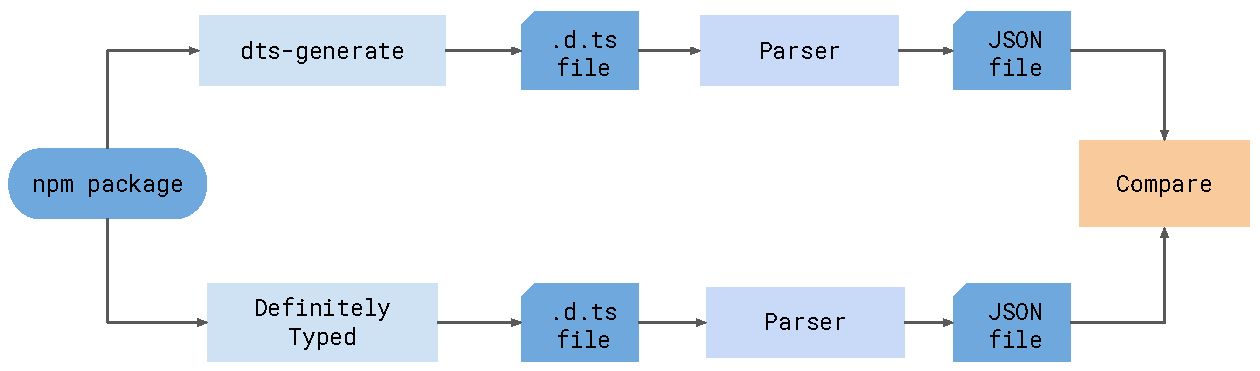
\includegraphics[width=1\textwidth]{evaluation-diagram.pdf}}
        \caption[Evaluation against DefinitelyTyped Repository]{\textbf{Evaluation of generated declaration files against DefinitelyTyped Repository} - A parser transforms the generated declaration file and the equivalent file in the DefinitelyTyped repository into a JSON file using the TypeScript Compiler API \cite{typescript-compiler-api}. Comparison is then performed on the JSON files, i.e. not on the declaration files.}
        \label{fig:evaluation-diagram}
    \end{centering}
\end{figure}

\subsection{dts-parse}
We need a means of comparing two declaration files. Of
course, we are not interested in a textual comparison, but in a
comparison of the structures described by the files.

The first step is to parse the declaration files, which can be
achieved by using the TypeScript Compiler API, a library which traverse the
Abstract Syntax Tree of a TypeScript program
\cite{typescript-compiler-api}. 
The step also performs a sanity check of the generated declaration
files as it rejects files with syntactic or semantics errors.
The output of \texttt{dts-parse} is a structure where declared
{interfaces}, {functions}, {classes} and
{namespaces} are stored separately. Function arguments are
correctly described, identifying complex types like union types or
callbacks. Optional parameters are also identified. For
{classes}, a distinction between the constructor and methods
is made. Declaration files are tagged according to their features, which is useful for identifying and filtering out declaration files containing unimplemented features.

\texttt{dts-parse} is itself written in TypeScript. It receives the file as input parameter and returns a JSON, as shown in \coderef{code:dts-parse-example}.

\begin{lstlisting}[
  caption={Example for \texttt{dts-parse} executed on module \texttt{glob-to-regexp} and combined with \texttt{jq} to browse through the returned JSON},
  language=bash,
label=code:dts-parse-example,
  float,
  abovecaptionskip=-\medskipamount
]
$ dts-parse -i glob-to-regexp/index.d.ts | jq '.parsing.functions[0].name'
"GlobToRegexp"
\end{lstlisting}

\subsection{dts-compare}
\label{sec:dts-compare}
The tool is written in TypeScript and receives 2 declaration files as an input and returns a JSON containing the result of the comparison, as shown in \coderef{code:dts-compare-example}. Following the naming convention of any standard Unit Testing framework, the input files are flagged as \lstinline{expected} or \lstinline{actual}. We assigned the \lstinline{expected} flag to the DefinitelyTyped declaration file.

\begin{lstlisting}[
  caption={Example for \texttt{dts-compare} executed on declaration files without differences},
  language=bash,
label=code:dts-compare-example,
  float,
  abovecaptionskip=-\medskipamount
]
$ dts-compare -e expected.d.ts -a actual.d.ts --module-name "my-module"
{
    "module": "my-module",
    "template": "module",
    "differences": [],
    "tags": []
}
\end{lstlisting}

\texttt{dts-compare} applies \texttt{dts-parse} internally to both files to get a common structure eligible for comparison. The result of the comparison is an array of an abstract entity called \texttt{Difference}. We extracted code examples written by developers to execute the code and gather run-time information. The quality of the generated declaration file is heavily dependent on the code examples. For example, if a property of an interface does not get accessed due to a code example not exploring a particular execution path, that property will not exist in the generated declaration file. Consequently, in order to isolate the impact of incomplete code examples on our quality analysis we identified each difference as follows:
\begin{itemize}
  \item \texttt{solvable}: Differences that can be solved by expanding the code examples. For example, invoking a function with different parameters so that a missing interface property gets accessed.
  \item \texttt{unsolvable}: Differences that can not be solved are marked as \texttt{unsolvable}. These differences are implementation errors of \texttt{dts-generate}.
\end{itemize}

The concrete evaluated differences are as follows:
\begin{itemize}
  \item \texttt{TemplateDifference}: A difference between the formal TypeScript templates. For example, if the file in DefinitelyTyped is written with \texttt{module} and we generated a file using \texttt{module-function}. The comparison stops if the templates differ.
  \item \texttt{ExportAssignmentDifference}: An equality check between the export assignments of both files, that is in the expression \lstinline{export = XXX}.
  \item \texttt{FunctionMissingDifference}: A function is present in the DefinitelyTyped file but not in the generated one. This applies to functions and methods of classes and interfaces.
  \item \texttt{FunctionMissingDifference}: A function is present in the generated declaration file but not in DefinitelyTyped.
  \item \texttt{FunctionOverloadingDifference}: The number of declarations for the same functions is different. This is particularly common when developers declare a function multiple times with different single types instead of using union types.
  \item \texttt{ParameterMissingDifference}: A parameter of a function or a property of an interface is not present in the generated file.
  \item \texttt{ParameterExtraDifference}: A parameter of a function or a property of an interface is present in the generated file but not in the DefinitelyTyped file.
  \item \texttt{ParameterTypeDifference}: A parameter of a function or a property of an interface is generated with a different type than in the DefinitelyTyped file. Here we differentiate between \texttt{SolvableDifference} and \texttt{UnsolvableDifference}.
  \begin{itemize}
    \item \texttt{SolvableDifference}: A type difference that can be solved by writing better code examples. This includes a basic type that is converted to a union type, a function overloading or a parameter or property that is marked as optional.
    \item \texttt{UnsolvableDifference}: Anything not considered as \texttt{SolvableDifference}.
  \end{itemize}
\end{itemize}

Type aliases are invisible to \texttt{dts-compare} as only final types were considered: the declaration \lstinline{type T = string | number; declare function F(a: T);} is equivalent to \lstinline{declare function F(a: string | number);}. The same concept applies for literal interfaces. \texttt{dts-compare} does not contemplate differences in function return types, since interface inference of function return types is not covered in this version of \texttt{dts-generate}.

\section{Results}
\label{sec:results}
We analyzed the obtained results focusing on the following aspects:
\begin{itemize}
  \item The quality of the inferred types, interfaces and module structure using runtime information.
  \item The benefits of using code examples provided by developers as a first approximation to execute the libraries and avoid a cold start problem.
  \item The usability of the generated declaration file and whether \texttt{dts-generate} can be used in a proper development environment.
\end{itemize}

\begin{quotation}
  The conducted experiments included tests that consisted of replacing
  a specific type definition from DefinitelyTyped
  \cite{definitely-typed-repository} with the one generated in the
  experiments: TypeScript compilation was successful, the generated
  JavaScript code ran without errors and code intelligence features
  performed by IDEs like code completion worked as expected.
\end{quotation}

Declaration files were generated for existing modules uploaded to the
\NPM{} registry. The DefinitelyTyped repository was used as a
benchmark. Each one of the generated files was compared against the
corresponding declaration file already uploaded to the repository.

Figure \ref{fig:experiments-overall-funnel} shows that a declaration
file was generated for 244 modules out of 6029 modules and we identified 80 modules that have only the features implemented by \texttt{dts-generate}. We obtained positive results for 69 of them. A detailed explanation of the overall quality of the generated files is provided in \secref{sec:experiments-evaluation}. Samples of the
generated declaration files for templates \textbf{module},
\textbf{module-class} and \textbf{module-function} are presented in
\secref{sec:experiments-declaration-files-generation}. 

\definecolor{myellow}{RGB}{228,212,0}
\definecolor{mgreen}{RGB}{5,104,57}

\newcommand\funnel[3]{%
\pgfmathsetmacro\mwid{(0.3+\val*0.06)}
\pgfmathsetmacro\mradius{(\val*0.01 + 1)}
\pgfmathsetmacro\mheight{(\val*0.003 + 0.4)}
\pgfmathsetmacro\marc{\mwid-.4}
    \begin{scope}[%
        shift={(0,#1)}, 
        line width=.05pt, 
        %x=5mm, 
        scale=0.7,
        yshift=\xi*0.05
        ]
    \draw[black,bottom color=#2, top color=#2] (-\mwid,0) -- (-\mwid+.4,-\mheight) arc (190:350:\marc cm and \mradius mm) -- (\mwid,0);
    \draw[black,fill=#3] (0,0) ellipse (\mwid cm and \mradius mm);
    \path (-\mwid,0) -- (-\mwid+.4,-\mheight) coordinate[midway] (a\xi);
    \end{scope}
}

\begin{figure}[tp]
	\hspace*{-0.16\textwidth}
	\centering
	\begin{tikzpicture}
		\foreach \val
				[%
				count=\xi starting from 0, 
				evaluate=\xi as \shadecolor using int(25*\xi),
				evaluate=\xi as \coord using int(\xi-12)
				]
			in {
				4.05,
				7.33,
				24.02,
				37.49,
				71.19,
				82.50,
				100.00
			}{
				\funnel{\coord}{mgreen!\shadecolor !myellow}{mgreen!\shadecolor !myellow}
			}   

		\node[left=0.02\textwidth of a0] {Generated Declaration Files};
		\node[right=0.04\textwidth of a0] {\textbf{244}};

		\node[left=0.02\textwidth of a1] {Run-time Information};
		\node[right=0.06\textwidth of a1] {\textbf{442}};

		\node[left=0.02\textwidth of a2] {Working Examples};
		\node[right=0.17\textwidth of a2] {\textbf{1448}};

		\node[left=0.02\textwidth of a3] {Code Examples};
		\node[right=0.25\textwidth of a3] {\textbf{2260}};

		\node[left=0.02\textwidth of a4] {README file};
		\node[right=0.45\textwidth of a4] {\textbf{4292}};

		\node[left=0.02\textwidth of a5] {Github Repository};
		\node[right=0.52\textwidth of a5] {\textbf{4974}};

		\node[align=right,left=0.02\textwidth of a6, text width=0.25\textwidth] {Definitely Typed Modules};
		\node[right=0.62\textwidth of a6] {\textbf{6029}};

	\end{tikzpicture}
	\caption[Number of analyzed modules for each stage of the experiment]{\textbf{Number of analyzed modules for each stage of the experiment} - A TypeScript Declaration File was generated for only 244 modules, out of 6029 modules in the DefinitelyTyped Repository. It was possible to gather valid run-time information for only 25\% of the modules for which a Code Example was extracted.}
	\label{fig:experiments-overall-funnel}
\end{figure}

\subsection{Code Examples}
Retrieving the code examples for the JavaScript libraries proved to be
a pragmatic way of driving the type gathering at run time. However, as
shown in \figref{fig:experiments-overall-funnel}, it was only possible
to obtain working code examples for 2260 packages. The
process of getting a valid code example for a module is divided in four
stages: 
\begin{itemize}
\item Extracting repository URL.
\item Extracting README file.
\item Extracting code examples from README files.
\item Executing code examples and discarding failing ones.
\end{itemize}

The results obtained for each on of them are described in the
following sections. 

\paragraph*{Repository URL}
The URL of the source repository could be retrieved for only 4974
packages. More than 1000 packages on \NPM{} do not have a repository
entry in their corresponding \texttt{package.json} file. Therefore, the
\texttt{npm view <module> repository.url} command returns no
value. Even important modules like \texttt{ace} provide no repository URL.

\paragraph*{README Files}
700 packages do not have a README file in their repository, although
the implementation checks for several naming conventions like
\texttt{readme.md} or \texttt{README.md}. 

\paragraph*{Extraction of Code Examples}
In this step, we loose another 50\% of modules! This loss is mainly
explained because some developers do not wrap their code in a block
using the \texttt{javascript} or \texttt{js} tags. However, as we are
still left with code examples for 2200 modules, we did not further
look into code extraction as this number was considered sufficient for
evaluating the generation of declaration files. 

\paragraph*{Execution of Code Examples}
We executed the remaining 2260 extracted code by installing the
required packages and running the code as a \NodeJS{}
application. Unfortunately, the code examples only worked for 1448
modules. 812 modules did not run correctly and had to be
discarded. Some failing samples were analyzed and there were mainly
two reasons for the failure: 
\begin{itemize}
\item The code fragment had been properly extracted but the code was
  not faulty. It was executing the library in an unsupported
  (obsolete?) way, which lead to a run-time error.
\item The extracted code fragment was not intended to be executed
  and/or it was not even valid JavaScript code. 
\end{itemize}

\paragraph*{Run-time Information}
Run-time information was extracted for only 442 out of 1448 modules with working code examples. As explained, in order to extract the run-time information, the behavior of the code under analysis was explicitly modified by wrapping the arguments around Wrapper Objects. Furthermore, Jalangi’s instrumentation itself caused some executions to fail, since the modules contained JavaScript features that are not supported by Jalangi. As a result, run-time information could not be extracted for 1006 modules. An instrumentation without user defined analysis modules was not applied, so it was not possible to determine which modules were failing only because of Jalangi’s own limitations.

\paragraph*{Generated Declaration Files}
A declaration file was generated for 244 out of 442 modules. Despite the correct execution of instrumented code examples, 198 modules did not contain suitable run-time information for generating a declaration file. The extracted code examples for these modules did not execute the library itself and therefore the collected run-time information was not useful for generating a declaration file.

\subsection{Declaration Files Generation}
\label{sec:experiments-declaration-files-generation}

This section exhibits some samples of the 244 generated
declaration files. It shows some results for each of the implemented
templates: \textbf{module}, \textbf{module-function} and
\textbf{module-class}. 

\figref{fig:experiments-results-module-function} shows the generated
declaration files for simple modules like \texttt{abs},
\texttt{dirname-regex}, and \texttt{escape-html}. All of them were
generated using the \textbf{module-function} template. Left side of the figure shows the generated declaration file with
\lstinline{dts-generate}, the right side shows the corresponding file
in the DefinitelyTyped repository. There are no relevant
differences between the files. Functions are correctly detected; input and output types are accurately inferred.


Differences in the export assignment by modules \texttt{dirname-regex} and \texttt{escape-html} is not problematic since the exported module can receive a custom name given by the developer. \texttt{dts-generate} automatically generates the export assignment by transforming the module name into camel case form, following TypeScript guidelines. The parameter names are extracted from the variable names of the JavaScript code. The JavaScript concrete implementation of module \texttt{escape-html} declares the first parameter of the exported function with the name \texttt{string} and not \texttt{text}, as specified in DefinitelyTyped. A difference in the names of the function parameters will anyway not affect the code compilation in any way. Furthermore, the omitted namespace in module \texttt{escape-html} is irrelevant. It is actually not required, since there is nothing declared within the namespace.
 
\begin{figure}[tp]
    \centering
    \begin{subfigure}{0.48\linewidth}
      \begin{lstlisting}[language=TypeScript]
export = Abs;

declare function Abs(input: string): string;
      \end{lstlisting}
      \caption{abs/index.d.ts - Generated}
    \end{subfigure}
    \hfill
    \begin{subfigure}{0.48\linewidth}
      \begin{lstlisting}[language=TypeScript]
declare function Abs(input: string): string;
export = Abs;
      \end{lstlisting}
      \caption{abs/index.d.ts - DefinitelyTyped}
    \end{subfigure}


    \begin{subfigure}{0.48\linewidth}
        \begin{lstlisting}[language=TypeScript]
export = DirnameRegex;

declare function DirnameRegex(): RegExp;
        \end{lstlisting}
        \caption{dirname-regex/index.d.ts - Generated}
      \end{subfigure}
      \hfill
      \begin{subfigure}{0.48\linewidth}
        \begin{lstlisting}[language=TypeScript]
export = dirnameRegex;

declare function dirnameRegex(): RegExp;
        \end{lstlisting}
        \caption{dirname-regex/index.d.ts - DefinitelyTyped}
      \end{subfigure}


      \begin{subfigure}{0.48\linewidth}
        \begin{lstlisting}[language=TypeScript]
export = EscapeHtml;

declare function EscapeHtml(string: string): string;
        \end{lstlisting}
        \caption{escape-html/index.d.ts - Generated}
      \end{subfigure}
      \hfill
      \begin{subfigure}{0.48\linewidth}
        \begin{lstlisting}[language=TypeScript]
declare function escapeHTML(text: string): string;
declare namespace escapeHTML { }

export = escapeHTML;
        \end{lstlisting}
        \caption{escape-html/index.d.ts - DefinitelyTyped}
      \end{subfigure}

    \caption{Results for \textbf{module-function} template}
    \label{fig:experiments-results-module-function}
\end{figure}
  

\begin{figure}[tp]
    \centering
    \begin{subfigure}{0.48\linewidth}
      \begin{lstlisting}[language=TypeScript]
export function v1(str: string): boolean;
export function v2(str: string): boolean;
export function v3(str: string): boolean;
export function v4(str: string): boolean;
export function v5(str: string): boolean;
      \end{lstlisting}
      \caption{is-uuid/index.d.ts - Generated}
    \end{subfigure}
    \hfill
    \begin{subfigure}{0.48\linewidth}
      \begin{lstlisting}[language=TypeScript]
export function v1(value: string): boolean;
export function v2(value: string): boolean;
export function v3(value: string): boolean;
export function v4(value: string): boolean;
export function v5(value: string): boolean;
export function nil(value: string): boolean;
export function anyNonNil(value: string): boolean;
      \end{lstlisting}
      \caption{is-uuid/index.d.ts - DefinitelyTyped}
    \end{subfigure}

    \caption{Results for \textbf{module}  module \texttt{is-uuid}}
    \label{fig:experiments-results-module-is-uuid}
\end{figure}

A sample for the \textbf{module} template
for the \texttt{is-uuid} module is shown in
\figref{fig:experiments-results-module-is-uuid}.
Again, methods that were not executed by the extracted examples are
not included in the declaration file. 

Finally, we could not generate a correct declaration file with the template \texttt{module-class}. All the modules corresponding to this template had at least one of the unimplemented TypeScript features.

It is worth mentioning that for some libraries the declaration file in
DefinitelyTyped was not correct. For example, for the module
\texttt{glob-base}, the parameter \texttt{basePath} is declared as optional in DefinitelyTyped. However, when invoking the function without that parameter an Error is thrown at runtime. The file generated by \texttt{dts-generate} will never mark the parameter as optional, as shown in \figref{fig:experiments-results-module-glob-base}. Function return types interfaces are not inferred by \texttt{dts-generate}. Parameter name is also inferred as \texttt{pattern} instead of \texttt{basePath}, since the JavaScript implementation declares the parameter as \texttt{pattern}, as shown in \figref{fig:subfloat-globbase-js-implementation}. We even discovered errors in the selected template in DefinitelyTyped. The module \texttt{smart-truncate} in DefinitelyTyped uses the \texttt{module} template, but \texttt{dts-generate} generates a file using the \texttt{module-function} template. We see in \coderef{code:experiments-results-module-smart-truncate} that the module is indeed exported as a function, as inferred by \texttt{dts-generate}.

\begin{figure}[tp]
    \centering
    \begin{subfigure}{0.48\linewidth}
      \begin{lstlisting}[language=TypeScript]
export = GlobBase;

declare function GlobBase(pattern: string): object;
      \end{lstlisting}
      \caption{glob-base/index.d.ts - Generated}
    \end{subfigure}
    \hfill
    \begin{subfigure}{0.48\linewidth}
      \begin{lstlisting}[language=TypeScript]
declare function globbase(basePath?: string): globbase.GlobBaseResult;

declare namespace globbase {
    interface GlobBaseResult {
        base: string;
        isGlob: boolean;
        glob: string;
    }
}

export = globbase;
      \end{lstlisting}
      \caption{glob-base/index.d.ts - DefinitelyTyped}
    \end{subfigure}

    \begin{subfigure}{0.48\linewidth}
      \begin{lstlisting}[language=JavaScript]
var globBase = require('glob-base');

globBase();

// Throws: TypeError: glob-base expects a string.
      \end{lstlisting}
      \caption{Code example invoking the exported function without the first parameter, as specified in DefinitelyTyped}
    \end{subfigure}
    \hfill
    \begin{subfigure}{0.48\linewidth}
      \begin{lstlisting}[language=TypeScript]
'use strict';

// ...

module.exports = function globBase(pattern) {
  if (typeof pattern !== 'string') {
    throw new TypeError('glob-base expects a string.');
  }

  // ...
} 
      \end{lstlisting}
      \caption{glob-base/index.js - Fraction of JS implementation that throws an Error when input parameter is not a string}
      \label{fig:subfloat-globbase-js-implementation}
    \end{subfigure}

    \caption{Incorrect optional parameter for module \texttt{glob-base}}
    \label{fig:experiments-results-module-glob-base}
\end{figure}

\begin{lstlisting}[
  caption={Code example for \texttt{smart-truncate} module exporting a function},
label=code:experiments-results-module-smart-truncate,
  language=JavaScript
]
var smartTruncate = require('smart-truncate');

var string = 'To iterate is human, to recurse divine.';

// Append an ellipsis at the end of the truncated string.
var truncated = smartTruncate(string, 15);
\end{lstlisting}

\subsection{Evaluation}
\label{sec:experiments-evaluation}
We analyzed only 82 of the 244 generated files. The remaining 162 files contained at least one of the unimplemented TypeScript features and were therefore not considered. These features were identified by \texttt{dts-parse} as tags.

As shown in \figref{fig:experiments-results-module-is-uuid}, the code examples have a direct influence on the quality of the generated declaration file. We introduced the concept of \texttt{solvable} and \texttt{unsolvable} differences in \secref{sec:dts-compare}. Modules containing only \texttt{solvable} differences were considered as positive results. We identified 72 such modules. We completed the examples manually for 10 of those modules, making them equivalent to the DefinitelyTyped files, as shown in \figref{fig:experiments-results-manually-completed-examples}. Expected differences are present: optional parameters are declared both with the actual and \texttt{undefined} type and the union type is handled through multiple overloads.

\begin{figure}[tp]
  \centering
  \begin{subfigure}{0.80\linewidth}
    \begin{lstlisting}[language=TypeScript]
declare namespace gh {
  interface Options {
      enterprise?: boolean;
  }
  interface Result {
      user: string;
      repo: string;
      branch: string;
      https_url: string;
      tarball_url: string;
      clone_url: string;
      travis_url: string;
      api_url: string;
      zip_url: string;
  }
}

declare function gh(url: string | {url: string}, options?: gh.Options): gh.Result | null;

export = gh;    
    \end{lstlisting}
    \caption{github-url-to-object/index.d.ts - DefinitelyTyped}
  \end{subfigure}

  \begin{subfigure}{0.80\linewidth}
    \begin{lstlisting}[language=TypeScript]
export = GithubUrlToObject;

declare function GithubUrlToObject(repoUrl: string|GithubUrlToObject.I__repoUrl, opts: undefined): object;
declare function GithubUrlToObject(repoUrl: string|GithubUrlToObject.I__repoUrl, opts: GithubUrlToObject.I__opts): null|object;
declare function GithubUrlToObject(repoUrl: GithubUrlToObject.I__repoUrl, opts: undefined): object;
declare namespace GithubUrlToObject {
  export interface I__repoUrl {
    'url': undefined | string;
  }

  export interface I__opts {
    'enterprise': undefined | boolean;
  }
}
    \end{lstlisting}
    \caption{github-url-to-object/index.d.ts - Generated with manually expanded code example}
  \end{subfigure}

  \begin{subfigure}{0.80\linewidth}
    \begin{lstlisting}[language=JavaScript]
var gh = require('github-url-to-object')

gh('github:monkey/business');
gh('https://github.com/monkey/business');
gh('https://github.com/monkey/business/tree/master');
gh('https://github.com/monkey/business/tree/master/nested/file.js');
gh('https://github.com/monkey/business.git');
gh('http://github.com/monkey/business');
gh('git://github.com/monkey/business.git');

// Manually added:
gh('git+https://githuuub.com/monkey/business.git', {});
gh('git+https://githuuub.com/monkey/business.git', {enterprise: true});
gh({url: 'git://github.com/monkey/business.git'});
      
    \end{lstlisting}
    \caption{Code example for module \texttt{github-url-to-object}.}
    \end{subfigure}
  \caption{Manually expanded code example for \texttt{github-url-to-object} to match DefinitelyTyped declaration file. Literal interface in DefinitelyTyped gets replace by a declared interface. The \texttt{undefined} type is used instead of the optional type. Return types are not considered.}
  \label{fig:experiments-results-manually-completed-examples}
\end{figure}

We identified only 10 modules with \texttt{unsolvable} differences. Most of them were caused for the same error: 8 modules had an incorrectly declared interface for the \texttt{string} type. This interface contained standard properties or methods from the JavaScript \texttt{String} object, such as \texttt{length} or \texttt{indexOf()}. The remaining modules are \texttt{duplexer2} and \texttt{duplexer3}. Both of them used native NodeJS types within the declaration file and \texttt{dts-generate} could not identify those properly.


\section{Related Work}
\label{sec:related-work}
\paragraph*{Microsoft's dts-gen}
Microsoft developed \texttt{dts-gen}, a tool that creates starter declaration files for JavaScript libraries \cite{dts-gen}. Its documentation states that the result is however intended to be only used a starting point. The outcome needs to be refined afterwards by the developers.

The tool analyzes the shape of the objects at runtime after initialization without executing the library. This results in many variables being inferred as \lstinline[language={}]{any}. \coderef{code:related-work-dts-gen-example} shows an example for module \lstinline[language={}]{abs}.

The solution presented in this work, however, is intended to generate declaration files that are ready to be uploaded to DefinitelyTyped without further manual intervention. Any amount of manual work that a developer needs to do on a declaration file after updating JavaScript code increases the risk for having discrepancies between the declaration file and the implementation.

Formal aspects like applying the right template and using the correct syntax are perfectly covered by \texttt{dts-gen}.

\begin{lstlisting}[
    language=bash,
    caption={Microsoft's dts-gen example - A declaration file for module \lstinline!abs! is generated. Types are inferred as \lstinline!any!. The correct \lstinline!module-function! template is used.},
	label=code:related-work-dts-gen-example,
    float,
    abovecaptionskip=-\medskipamount
]
$ npm i -g dts-gen
$ npm i -g abs
$ dts-gen -m abs
Wrote 5 lines to abs.d.ts.

$ cat abs.d.ts
/** Declaration file generated by dts-gen */

export = abs;

declare function abs(input: any): any;
\end{lstlisting}

\paragraph*{TSInfer \& TSEvolve}
TSInfer and TSEvolve are presented as part of TSTools \cite{DBLP:conf/fase/KristensenM17}. Both tools are the continuation of TSCheck \cite{DBLP:conf/oopsla/FeldthausM14}, a tool for looking for mismatches between a declaration file and an implementation.

TSInfer proceeds in a similar way than TSCheck. It initializes the library in a browser and it records a snapshot of the resulting state and then it performs a light weight static analysis on all the functions and objects stored in the snapshot.

The abstraction and the constraints they introduced as part of the static analysis tools for inferring the types have room for improvement. A run-time based approach like the one presented in our work will provide more accurate information, thus generating more precise declaration files.

Since they analyze the objects and functions stored in the snapshot, they faced the problem of including in the declaration file internal methods and properties that developers wanted to hide. Run-time information would have informed that the developer has no intention of exposing such methods.

Moreover, TSEvolve performs a differential analysis on the changes made to a JavaScript library in order to determine intentional discrepancies between declaration files of two consecutive versions. We consider that a differential analysis may not be needed. If the developer's intention is accurately extracted and the execution code clearly represents that intention then the generated declaration file would already describe the newer version of a library without the need of a differential analysis.

\paragraph*{TSTest}
TSTest is a tool that checks for mismatches between a declaration file and a JavaScript implementation \cite{DBLP:journals/pacmpl/KristensenM17}. It applies feedback-directed random testing for generating type test scripts. These scripts will execute the library in order to check if it behaves the way it is described in the declaration file. TSTest also provides concrete executions for mismatches.

We evaluated the generated declaration files comparing them to the declaration files uploaded to DefinitelyTyped. The disadvantage of doing this is that since the uploaded files are written manually, they could already contain mismatches with the JavaScript implementation. However, it is a suitable choice for a development stage since it is used as a baseline.

In a final stage, declaration files need to be checked against the proper JavaScript implementation and TSTest has to be definitely taken into account.

\section{Conclusion}
\label{sec:conclusion}
We have presented \texttt{dts-generate}, a tool for generating a TypeScript declaration file for a specific JavaScript library. The tool downloads code samples written by the developers from the library's repository. It uses these samples to execute the library and gather data flow and type information. The tool finally generates a TypeScript declaration file based on the information gathered at run-time.

We developed an architecture that supports the automatic generation of declaration files for specific JavaScript libraries without additional manual tasks. The architecture contemplates a future incorporation of a Symbolic Execution Engine that refines the initial code base enabling the exploration of new execution paths. However not implemented in this work, its incorporation would result in small incremental modifications to the presented architecture as it is considered to only expand the existing code base.

Building an end-to-end solution for the generation of TypeScript declaration files was prioritized over type inference accuracy. Consequently, types were taken over from the values at run-time. Since developers expose through code how a library should be used, obtaining the types from the code examples extracted from the repositories proved to be a pragmatic and effective approximation, enabling to work on specific aspects regarding the TypeScript declaration file generation itself.

We built a mechanism to automatically create declaration files for potentially every module uploaded to DefinitelyTyped. We managed to generate declaration files for 244 modules. We compared the results against the corresponding files uploaded to DefinitelyTyped by creating \texttt{dts-parse}, a TypeScript declaration files parser and \texttt{dts-compare}, a comparator.

We exposed the fundamental aspect of capturing the developer's intention when inferring types in JavaScript. Instead of applying constraints and restrictions for operations with certain types, we presented a proposal where common practices are favored. Uncommon usage is not forbidden but greatly disfavored. Accordingly, we collected evidence regarding the usage of JavaScript operators by analyzing 400 libraries.

Finally, the architecture is composed of different blocks that interact with each other. Each block is independent and has a well defined behavior as well as clear input and output values. As a result, each block can be independently and simultaneously improved.


\bibliography{main}

\end{document}
